\chapter{Desenvolvimento e Arquitetura do Sistema}
\label{cap:arquitetura}

O Sistema de Realidade Virtual para Treinamento de Segurança em Canteiro de Obras foi desenvolvido em Unity 6 LTS com o Meta XR SDK, para execução no Meta Quest 3 com rastreamento de mãos como modalidade primária de entrada. A arquitetura atende a dois propósitos: criar e executar cenários de treinamento baseados em situações críticas reais da construção civil e avaliar de forma sistemática o desempenho do usuário, com foco na identificação de comportamentos seguros diante dos riscos simulados.

Em vez de concentrar interação, renderização, gerência de estado e avaliação de regras nos mesmos componentes --- prática comum em protótipos de motor de jogo, mas que dificulta manutenção e evolução ---, o sistema adota uma \gls{EDA}. A lógica de domínio reside em classes C\# puras, independentes do motor (sufixo \texttt{Core}), envolvidas por adaptadores \texttt{MonoBehaviour} que fazem a ponte com a cena, seguindo o padrão \textit{ports-and-adapters}. As camadas coordenam-se por meio de eventos tipados publicados em um barramento central, sem manter referências diretas entre si. Essa separação sustenta a testabilidade, a resiliência a atualizações de \gls{SDK} e a autoria de cenários sem alteração de código, propriedades retomadas no Capítulo~\ref{cap:validacao}.

\section{Visão Geral em Camadas}

A arquitetura organiza o sistema em sete camadas conectadas por um \texttt{EventBus} tipado, que atua como espinha de comunicação (Figura~\ref{fig:arquitetura}). As camadas vão da configuração de dados, na base, à publicação de eventos, ao núcleo de domínio, à interface reativa e à saída em rede, no topo. O acoplamento ao SDK fica confinado às camadas de publicação e de adaptadores; o núcleo de domínio, o subsistema de avaliação e a interface não possuem dependências do motor.

\begin{figure}[htb]
    \centering
    \caption{Arquitetura em camadas orientada a eventos do sistema de treinamento. MB: \texttt{MonoBehaviour}.}
    \label{fig:arquitetura}
    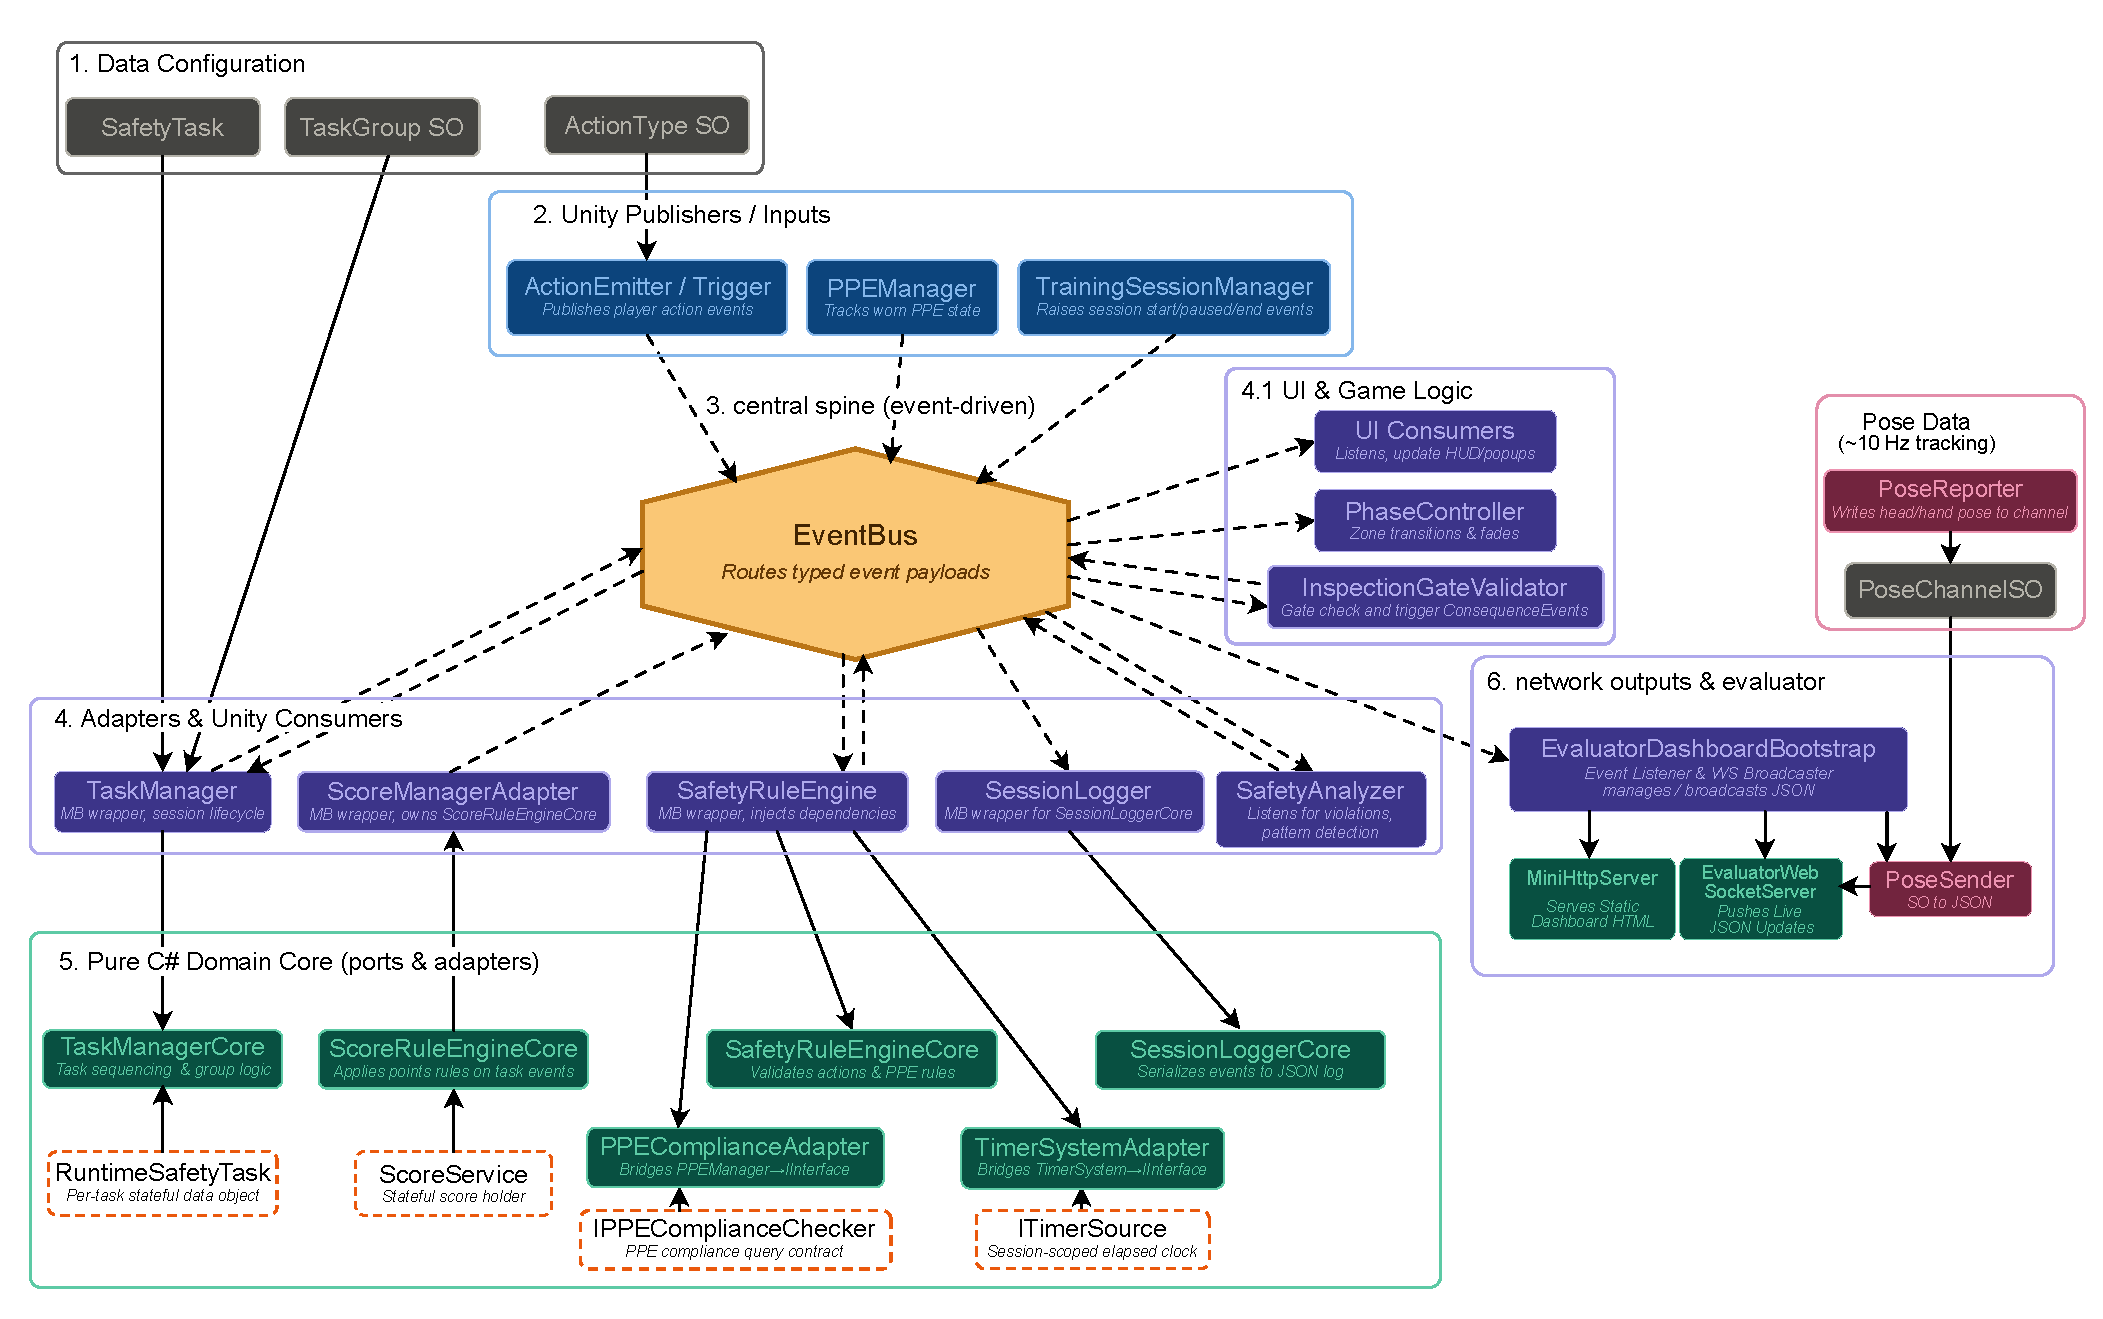
\includegraphics[width=\textwidth]{figuras/safety-proto-architecture}

    {\footnotesize Fonte: elaborado pelo autor.}
\end{figure}

\section{Camadas da Arquitetura}

\textbf{Camada 1 -- Configuração de Dados.} O conteúdo dos cenários reside em \textit{assets} nativos do editor (\texttt{ScriptableObject}), e não em código. Três tipos compõem a camada: \texttt{SafetyTask}, que descreve uma ação treinável e suas regras de pontuação; \texttt{TaskGroup}, que agrupa tarefas sob um modo de execução (sequencial ou ordem livre) e pode declarar dependências entre grupos; e \texttt{ActionType}, que define o vocabulário canônico de interações ligando objetos da cena às expectativas das tarefas. Como consequência, a autoria de cenários dispensa alteração de código e os cenários são versionados como \textit{assets}, com fluxo padrão de \textit{diff}, ramificação e revisão.

\textbf{Camada 2 -- Publicadores.} Traduz a interação física do jogador e o ciclo de vida da sessão em eventos tipados. Seus componentes são produtores puros: nunca assinam eventos. Produtores de ação emitem um evento canônico quando o jogador interage com um objeto (preensão, proximidade ou \textit{callback} do SDK de interação); o \texttt{PPEManager} publica mudanças de estado dos EPIs; e o \texttt{TrainingSessionManager} emite eventos de ciclo de sessão (início, pausa, retomada, término).

\textbf{Camada 3 -- Barramento Central.} O \texttt{EventBus} é o único \textit{broker} tipado de publicação/assinatura pelo qual fluem todas as interações entre camadas. Ele expõe primitivas genéricas de assinatura e publicação parametrizadas pelo tipo da carga do evento e processa sua fila uma vez por quadro, garantindo ordem de despacho consistente com o ciclo de atualização do motor.

\textbf{Camada 4 -- Adaptadores.} É a costura entre o motor e o núcleo independente. Cada núcleo de domínio possui um invólucro que assina o barramento, encaminha eventos para o núcleo e publica de volta os resultados. Componentes que legitimamente exigem serviços do motor --- transições de cena, esmaecimento de tela --- consomem o barramento diretamente. A injeção de dependências concentra-se aqui, e o risco de migração de SDK fica contido nesta camada e na de publicadores.

\textbf{Camada 5 -- Núcleo de Domínio (C\# puro).} É onde as principais propriedades arquiteturais são testáveis, pois suas classes não têm dependências do motor. O \texttt{TaskManagerCore} gerencia o sequenciamento de tarefas e grupos, trata dependências, \textit{timeouts} e violações de ordem nos modos sequencial e de ordem livre. O \texttt{SafetyRuleEngineCore} valida cada ação contra as tarefas ativas e verifica conformidade dos EPIs, emitindo evento de violação quando uma restrição normativa é quebrada. O \texttt{ScoreRuleEngineCore} aplica regras de pontuação e penalidade, mantendo a política de escore dentro do núcleo. O \texttt{SessionLoggerCore} assina todos os eventos do barramento e, ao final, serializa o histórico por meio de uma estratégia injetada por dependência.

\textbf{Camada 6 -- Interface do Usuário.} É puramente reativa: nenhum componente publica eventos ou mantém estado de domínio; cada um assina o barramento e apenas atualiza a exibição. As superfícies em cena incluem um HUD de pontuação, um cronômetro por tarefa, um painel de progresso de tarefa e grupo, um resumo de conclusão de sessão e avisos contextuais. Como a interface consome o mesmo protocolo de eventos das demais camadas, apresentações alternativas (um painel \textit{desktop}, uma visão de espectador) podem ser introduzidas sem alterar produtores ou núcleo de domínio.

\textbf{Camada 7 -- Saída em Rede e Painel do Avaliador.} Permite a observação remota, em tempo real, por instrutor ou pesquisador na rede local, sem intervir na simulação. Um componente de \textit{bootstrap} inicia um servidor HTTP (página estática do painel) e um servidor WebSocket (transmissão de eventos ao vivo) na inicialização do dispositivo, assina todos os eventos do barramento e os retransmite em \gls{JSON} para os navegadores conectados. Dados de pose de alta frequência (cabeça, mãos e objetos de EPI, a cerca de 10~Hz) trafegam por um canal dedicado, separado do canal de eventos discretos, para não congestioná-lo.

\section{Catálogo de Eventos}

O protótipo define 18 eventos lógicos, dos quais 16 são despachados como canais tipados do \texttt{EventBus}, implementados por 13 classes de carga (eventos correlatos compartilham uma classe distinguida por um \textit{enum} de fase). Os módulos nunca inspecionam entrada bruta nem consultam estado externo diretamente. A Tabela~\ref{tab:eventos} resume os grupos de eventos e seus principais publicadores.

\begin{table}[htb]
    \centering
    \caption{Grupos de eventos do protótipo e seus principais publicadores.}
    \label{tab:eventos}
    \begin{tabular}{lll}
        \toprule
        \textbf{Grupo} & \textbf{Eventos representativos} & \textbf{Publicador} \\
        \midrule
        Ciclo de sessão   & \texttt{SessionStarted}/\texttt{Completed} & \texttt{TrainingSessionManager} \\
        Interação         & \texttt{ActionAttempt}                     & \texttt{ActionEmitter} \\
        Conformidade EPI  & \texttt{PpeStateChanged}                   & \texttt{PPEManager} \\
        Tarefas e grupos  & \texttt{TaskStarted}/\texttt{Completed}    & \texttt{TaskManagerCore} \\
        Pontuação         & \texttt{ScoreChanged}                      & \texttt{ScoreService} \\
        Análise de risco  & \texttt{SafetyViolation}                   & \texttt{SafetyRuleEngineCore} \\
        \bottomrule
    \end{tabular}

    {\footnotesize Fonte: elaborado pelo autor.}
\end{table}

\section{Ciclo de Vida das Tarefas}

O \texttt{TaskManagerCore} avança a tarefa correspondente a cada evento de interação e publica o evento de ciclo de vida de volta no barramento. A Figura~\ref{fig:lifecycle} ilustra a máquina de estados resultante para os modos sequencial e de ordem livre: toda transição de estado é publicada como evento tipado, sem que nenhum componente mantenha referência direta ao \texttt{TaskManagerCore}.

\begin{figure}[htb]
    \centering
    \caption{Máquina de estados do ciclo de vida das tarefas nos modos sequencial e de ordem livre. Os círculos numerados traçam o caminho canônico de sucesso.}
    \label{fig:lifecycle}
    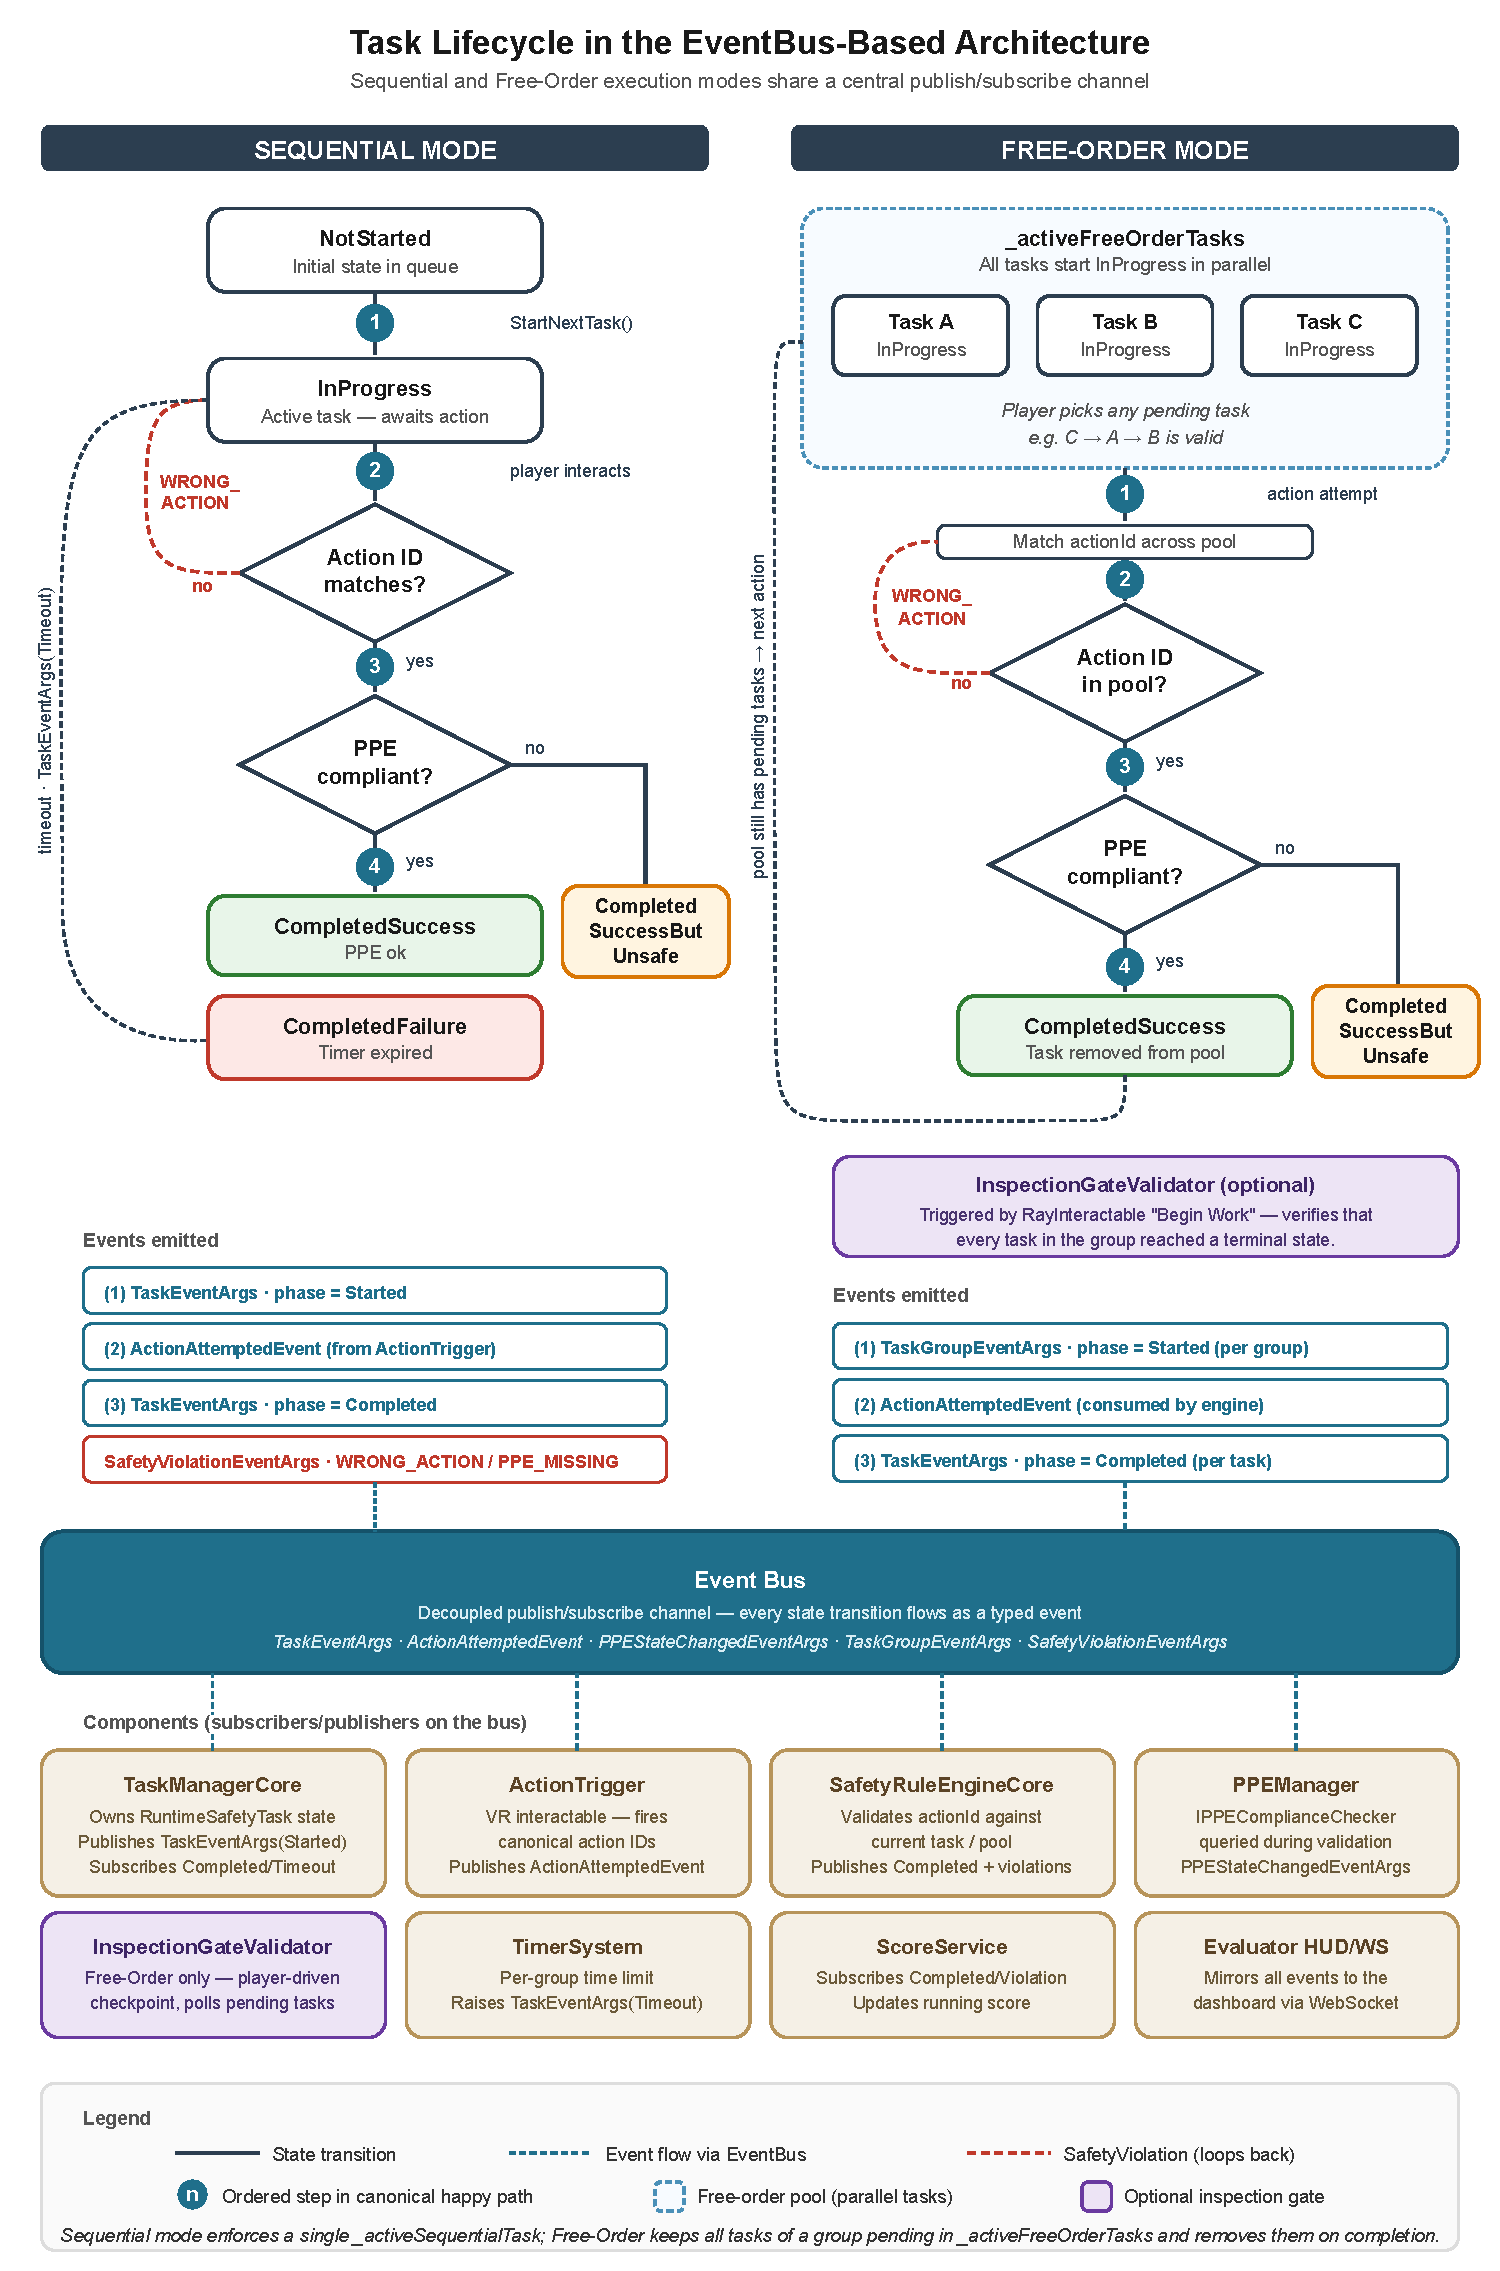
\includegraphics[width=0.85\textwidth]{figuras/task_lifecycle_vertical}

    {\footnotesize Fonte: elaborado pelo autor.}
\end{figure}

\section{Subsistema de Avaliação de Desempenho}

O subsistema de avaliação monitora, registra e analisa o desempenho dos participantes durante a execução das tarefas. Ele opera sobre o mesmo protocolo de eventos das demais camadas, o que o torna exercitável fora do motor.

\subsection{Coleta de Dados em Tempo Real}

Eventos relevantes são capturados pelo barramento à medida que ocorrem: tentativas de ação (\texttt{ActionAttempt}), conclusão ou expiração de tarefas (\texttt{TaskCompleted}, \texttt{TaskTimeout}), mudanças de estado dos EPIs (\texttt{PpeStateChanged}) e término da sessão (\texttt{SessionCompleted}). Módulos especializados interceptam esses eventos e os encaminham aos sistemas de pontuação e \textit{feedback}.

\subsection{Pontuação e Desempenho}

A avaliação quantitativa decorre de dois componentes. O \texttt{ScoreService} é um detentor de escore que expõe primitivas de mutação e notificação, mas não assina o barramento --- o que permite testá-lo isoladamente. O \texttt{ScoreRuleEngineCore} escuta os eventos de ciclo de vida das tarefas e aplica pontuação ou penalidade segundo as regras definidas nos \textit{assets} \texttt{SafetyTask}. A pontuação é atualizada em tempo real, exibida no HUD e consolidada ao final da simulação.

\subsection{Monitoramento e Exportação de Dados}

Para análise posterior, o \texttt{SessionLoggerCore} registra todos os eventos relevantes da sessão com marcação temporal e gera um arquivo \gls{JSON} com o histórico de interações e um sumário de desempenho (tempo total, tarefas concluídas, pontuação). A esse registro somam-se \textit{logs} de interação (tempo por área, número de erros, decisões tomadas) e, mediante consentimento, a gravação de vídeo da sessão para avaliação qualitativa. Os identificadores de sessão são vinculados aos dados coletados para garantir rastreabilidade entre os \textit{logs} do sistema e os questionários externos (SUS e IPQ).

\section{Racional Arquitetural}

Cinco decisões merecem justificativa.

\textbf{Eventos tipados em vez de mensagens por chave textual.} Cargas tipadas eliminam erros de execução por digitação e permitem verificação em tempo de compilação; a migração de chaves textuais resolveu três defeitos latentes de incompatibilidade entre assinantes detectados na integração.

\textbf{\texttt{ScriptableObjects} como espinha de dados.} Arquivos JSON ou XML exigiriam analisadores e ferramental próprios. Os \textit{assets} \texttt{ScriptableObject} usam o inspetor nativo, o controle de versão e a serialização do Unity, sem infraestrutura adicional.

\textbf{Acoplamento de SDK confinado às bordas.} O núcleo de domínio, o subsistema de avaliação e a interface não têm dependências do SDK. O acoplamento concentra-se nas camadas de publicadores e adaptadores, de modo que mudanças incompatíveis do SDK afetam apenas essas bordas --- o que também viabiliza substituir a entrada de RV por um leitor de console na validação técnica.

\textbf{Serialização injetada como estratégia.} O \texttt{SessionLoggerCore} recebe sua estratégia de serialização por injeção de dependência, e não embutida, permitindo implementações específicas de contexto sem modificar a lógica central.

\textbf{Despacho com orçamento de quadro.} Aplicações de RV \textit{standalone} operam sob orçamentos rígidos de CPU. O \texttt{EventBus} limita o despacho por quadro e desvia os dados de pose de alta frequência para um canal próprio, evitando que a telemetria contínua concorra com os eventos de jogo.

\section{Generalidade e Extensibilidade}

Como a lógica de domínio é independente do motor e os cenários são definidos por dados, a arquitetura oferece \textit{afordância} para múltiplos domínios de treinamento além da construção civil --- por exemplo, procedimentos clínicos, montagem industrial ou resposta a emergências. Trata-se de uma propriedade de projeto: o protótipo foi implementado e validado apenas no domínio de construção sob a NR-18 e a NR-35, e a transferência empírica para outros contextos regulatórios permanece como trabalho futuro. No mesmo sentido, um \textit{backend} distribuído poderia sustentar sessões multiusuário substituindo o \texttt{EventBus} em processo, sem alterar as camadas de aplicação.
